\documentclass[notitlepage]{revtex4-2}
% includes...
\usepackage{amsmath}
\usepackage{bm}
\usepackage{natbib}
\usepackage{graphicx}
\usepackage{hyperref}
\usepackage{epstopdf}
\usepackage{color}
\usepackage{tikz}
\usetikzlibrary{arrows.meta}
\tikzset{%
  >={Latex[width=2mm,length=2mm]},
  % Specifications for style of nodes:
            base/.style = {rectangle, rounded corners, draw=black,
                           minimum width=2.5cm, minimum height=1cm,
                           text centered, font=\sffamily},
             box/.style = {base, fill=yellow!60, font=\scriptsize},
            boxs/.style = {base, fill=red!60, font=\tiny},
    activityRuns/.style = {base, fill=green!30},
         process/.style = {base, minimum width=2.5cm, fill=orange!15,
                           font=\ttfamily}

}
\begin{document}
%front matter
\title{SUNSET code: Scalable Unstructred Node-SET code for high fidelity fluid simulations in complex geometries}

\author{J. R. C. King}
\email{jack.king@manchester.ac.uk}
\affiliation{Department of Mechanical, Aerospace and Civil Engineering, The University of Manchester, Manchester, M13 9PL, UK}
\date{\today}
\begin{abstract}

This document contains a brief description and guide to the SUNSET code. Numerical methods in this code follow~\cite{king_labfm_2022} (also available at arXiv:2102.02019).

\end{abstract}

\maketitle
%end front matter

\section{Directory structure}




\section{Governing Equations}\label{ge}

The code solves the compressible Navier-Stokes equations in the form
\begin{equation}\frac{\partial\ln\rho}{\partial{t}}+\bm{u}\cdot\nabla\ln\rho=-\nabla\cdot\bm{u}\label{eq:mass}\end{equation}
\begin{equation}\frac{\partial\bm{u}}{\partial{t}}+\bm{u}\cdot\nabla\bm{u}=-\frac{1}{\rho}\nabla{p}+\frac{1}{\rho}\nabla\cdot\bm{\tau}+\bm{f}\label{eq:mom}\end{equation}
\begin{equation}\frac{\partial\rho{E}}{\partial{t}}+\bm{u}\cdot\nabla\left(\rho{E}\right)=-\nabla\cdot\left(p\bm{u}\right)-\nabla\cdot\bm{q}+\nabla\cdot\left(\bm{\tau}\bm{u}\right)+\bm{u}\cdot\bm{f}\label{eq:en}\end{equation}
and
\begin{equation}\frac{\partial{Y}_{\alpha}}{\partial{t}}+\bm{u}\cdot\nabla{Y}_{\alpha}=\frac{\dot\omega_{\alpha}}{\rho}-\frac{1}{\rho}\nabla\left(\rho\bm{V}_{\alpha}Y_{\alpha}\right)\qquad\forall\alpha\in\left[1,N_{S}\right]\label{eq:Y}\end{equation}
where $\rho$ is the density, $\bm{u}$ the velocity, $p$ the pressure, $E$ the total energy, $\bm{\tau}$ the viscous stress, $\bm{f}$ a body force, $\bm{q}$ the heat flux, $Y_{\alpha}$ the concentration of species $\alpha\in\left[1,N_{S}\right]$, and $\bm{V}_{\alpha}$ is the molecular diffusion velocity of species $\alpha$. $\dot\omega_{\alpha}$ is the production rate of species $\alpha$.

The viscous stress is defined as 
\begin{equation}\bm{\tau}=\mu\left(\nabla\bm{u}+\nabla\bm{u}^{T}-\frac{2}{3}\bm{I}\nabla\cdot\bm{u}\right)\label{eq:tau},\end{equation}
where $\mu$ is the dynamic viscosity and $\bm{I}$ is the identity tensor. The energy is
\begin{equation}E=\displaystyle\sum_{\alpha}h_{\alpha}Y_{\alpha}-\frac{p}{\rho}+\frac{1}{2}\bm{u}\cdot\bm{u}\label{eq:E}\end{equation}
where the sum over $\alpha$ is over all $\alpha\in\left[1,N_{S}\right]$, and $h_{\alpha}$ is the enthalpy of species $\alpha$, given by
\begin{equation}h_{\alpha}=\displaystyle\int_{T_{ref}}^{T}c_{p,\alpha}dT + h_{\alpha,ref}\label{eq:h}\end{equation}
with $h_{\alpha,ref}$ the enthalpy of species $\alpha$ at the reference temperature $T_{ref}$, and $c_{p,\alpha}$ the specific heat capacity at constant pressure of species $\alpha$, which in general may be a function of temperature $T$.
The molecular diffusion term in~\eqref{eq:Y} is modelled as a Fickian diffusion process with
\begin{equation}-\rho\bm{V}_{\alpha}Y_{\alpha}=\rho{D}_{\alpha}\nabla{Y}_{\alpha}-Y_{\alpha}\displaystyle\sum_{\beta\in\left[1,N_{S}\right]}\rho{D}_{\beta}\nabla{Y}_{\beta}\label{eq:fickdiff},\end{equation}
in which $D_{\alpha}$ is the molecular diffusivity of species $\alpha$, and the final term is a correction to ensure that 
\begin{equation}\displaystyle\sum_{\alpha}Y_{\alpha}=1.\end{equation}
The heat flux vector $\bm{q}$ is then given by
\begin{equation}\bm{q}=-\lambda\nabla{T}+\displaystyle\sum_{\alpha}\rho\bm{V}_{\alpha}Y_{\alpha}h_{\alpha}\label{eq:hfv},\end{equation}
where $\lambda$ is the thermal conductivity of the mixture.
The system is closed with an ideal gas equation of state
\begin{equation}p=\rho{R}_{mix}T=\rho{R}_{0}T\displaystyle\sum_{\alpha}\frac{Y_{\alpha}}{W_{\alpha}}\label{eq:eos}\end{equation}
where $R_{mix}$ is the gas constant for the mixture, $R_{0}$ is the universal gas constant, and $W_{\alpha}$ is the molar mass of species $\alpha$.

\subsection{Evaluation of temperature and heat capacity}

TBC.

TBC for cp independent of T.

\subsection{Temperature dependent transport properties}

The temperature dependence of the transport properties is modelled by the relationship
\begin{equation}\mu=\mu_{ref}\left(\frac{T}{T_{ref}}\right)^{r_{T}},\label{eq:tdtp_mu}\end{equation}
where $\mu_{ref}$ is the viscosity at the reference temperature $T_{ref}$, and $r_{T}=0.7$ is a constant exponent. The mixture thermal conductivity is given by
\begin{equation}\lambda=\frac{\mu}{c_{p}Pr},\end{equation}
in which $c_{p}$ is the heat capacity of the mixture, and $Pr$ is the Prandtl number, taken as constant. The molecular diffusivity of species $\alpha$ is given by
\begin{equation}D_{\alpha}=\frac{\lambda}{\rho{c}_{p}Le_{\alpha}},\end{equation}
where $Le_{\alpha}$ is the Lewis number for species $\alpha$, which is assumed constant for each species.

\subsection{Evaluation of reaction rates}

TBC.


\section{Numerical implementation}

\subsection{Basic framework and principles}

The domain is discretised with an unstructured node-set. Each node (or collocation point) $i$ has position $\bm{r}_{i}$, discretisation length-scale $s_{i}$ (the average local inter-node spacing), and holds the primary variables $\ln\rho_{i}$, $\bm{u}_{i}$, $\rho{E}_{i}$. The governing equations are solved on the set of nodes. Spatial derivatives are evaluated using LABFM~\cite{king_labfm_2022} in the first two dimensions ($x,y$) and high-order finite differences (FD) in the third dimension ($z$). Technically, the node-set is semi-unstructured...

Time integration is by third-order Runge-Kutta scheme. The solution is de-aliased with a high-order LABFM+FD filter after each time step~\cite{king_labfm_2022}. The accuracy of the spatial discretisation can be changed through compiler flags, between $4^{th}$ and $12^{th}$ order accurate in space. In typical usage, $8^{th}$ order provides a good compromise between accuracy and cost.

At wall, inflow and outflow boundaries, the node-set is structured, with a band of $5$ rows of uniformly spaced nodes. Wall boundaries may be curved, but \emph{at present,} must have uniform resolution along their length. On boundaries (and within the first $2$ rows of uniform nodes) the derivatives and filters in the $x-y$ plane are calculated through combinations of FD (normal to boundaries), one-dimensional LABFM (tangential to boundaries), and 2D LABFM. Details in~\cite{king_labfm_2022}.

Aside from the complexities of indexing and derivative evaluation associated with the unstructured node-set approach, the framework is similar to a high-order (central) finite difference scheme.

\subsection{Evaluation of derivatives}

Derivatives of the primary variables $\ln\rho$, $\bm{u}$, $\rho{E}$ and $Y_{\alpha}$ are evaluated with the LABFM method~\cite{king_labfm_2022}. Temperature gradients $\nabla{T}$ are also evaluated using LABFM, as are Laplacians where required (i.e. $\nabla^{2}\bm{u}$, $\nabla^{2}{T}$, $\nabla^{2}Y_{\alpha}$). 

To avoid the explicit evaluation of cross-second derivatives of velocity (which appear in the terms $\nabla\cdot\bm{\tau}$ and $\nabla\cdot\left(\bm{\tau}\bm{u}\right)$), these terms are constructed by evaluating the gradient of the velocity divergence $\nabla\cdot\bm{u}$.

The evaluation of derivatives using LABFM constitutes the bulk of the computational cost, and it is hence desirable avoid where possible. Gradients of secondary properties may be evaluated from analytic expressions as follows. The pressure gradient is calculated from the temperature gradient as 
\begin{equation}\nabla{p}=p\left(\frac{R_{0}}{R_{mix}}\displaystyle\sum_{\alpha}\frac{\nabla{Y}_{\alpha}}{W_{\alpha}}+\frac{1}{T}\nabla{T}+\nabla\ln\rho\right).\label{eq:gradp}\end{equation}
Gradients of mixture specific heat capacity and enthalpy are also evaluated through analytic expressions in terms of temperature gradients TBC.
Similarly, the gradients of the transport properties, which have analytic relations with the thermodynamic quantities, are evaluated as
\begin{equation}\nabla\mu=\frac{r_{T}\mu}{T}\nabla{T}\end{equation}
\begin{equation}\nabla\lambda=\frac{r_{T}\lambda}{T}\nabla{T}+\frac{\lambda}{c_{p}}\nabla{c_{p}}\end{equation}
\begin{equation}\nabla{D}_{\alpha}=\frac{r_{T}D_{\alpha}}{T}\nabla{T}-D_{\alpha}\nabla\ln\rho\end{equation}

\subsection{Boundaries}

Symmetry and periodic boundary conditions are available. The only boundary condition available in the third dimension is periodic. Wall, inflow and outflow boundaries are imposed through the Navier-Stokes characteristic boundary condition formalism of [citeXX]. The basic framework follows that described for isothermal flows in~\cite{king_labfm_2022}.

\subsection{Parallelisation}

The code is accelerated with a shared-distributed framework, using both OpenMP and MPI. It should be noted that the parallel efficiency of the OpenMP is low, due to memory-access issues. Provided sufficient memory is available, it is therefore recommended to run the code with very few threads per MPI rank: ideally $1$, but any more than $\approx{5}$ and resources are being used inefficiently.

Domain decomposition is three-dimensional, and \emph{currently} static. The total number of MPI ranks is $N_{p}=N_{px}N_{py}N_{pz}$, where the subscripts $x$, $y$ and $z$ indicate the number of ranks in each direction. The physical sizes of the subdomains are adjusted such that each MPI rank contains the same number of collocation points, resulting in approximate load balancing. On simple domains the parallel efficiency is $>96\%$ at $1024$ MPI ranks (relative to $4$ MPI ranks).

The domain-decomposition is likely to be restructured in the coming year, so I'll leave further details for now.

\section{Generating input files}


THIS SECTION TBC. CURRENTLY BASED ON OLD BUBBLY CODE

Input files are generated using the program \verb|gen2d|, found in \verb|source/gen/|. Navigate here then
\begin{verbatim}
make
./gen2d
cp I* ../../.
\end{verbatim}
When \verb|gen2d| is run, a list of cases is displayed. Input a number to specify a case. Once generated, you can use the command \verb|cp I* ../../.| to copy the case files \verb|INDAT|, \verb|IPART|, and \verb|IBOUND| to the main directory. Cases are hard-coded in the program \verb|gen2d|. To modify them, or create new cases, you need to modify the file \verb|datclass.F90|, and recompile with \verb|make|.

Within each case in \verb|datclass.F90|, domain sizes (\verb|xl|, \verb|yl|, and \verb|h0|) are specified, along with the resolution. Then dimensionless parameters are specified. Followed by boundary conditions (described below), and then the specification of the initial particle distribution. Note that entire problem is non-dimensionalised, so the domain specification and intitial velocity fields should have characteristic scales of unity. Also note that \verb|gen2d| generates two-dimensional case files, and a parameter \verb|nz| which specifies the number of particles in the third dimension (if a three-dimensional simulation is run).

The following cases are currently included in \verb|datclass.F90|:
\begin{enumerate}
\item Still water/bubble column
\item Dam Break (Lobovsky)
\item Taylor-Green
\item Poiseuille/channel flow
\item Third order Stokes wave
\end{enumerate}

\subsection{Boundary framework}


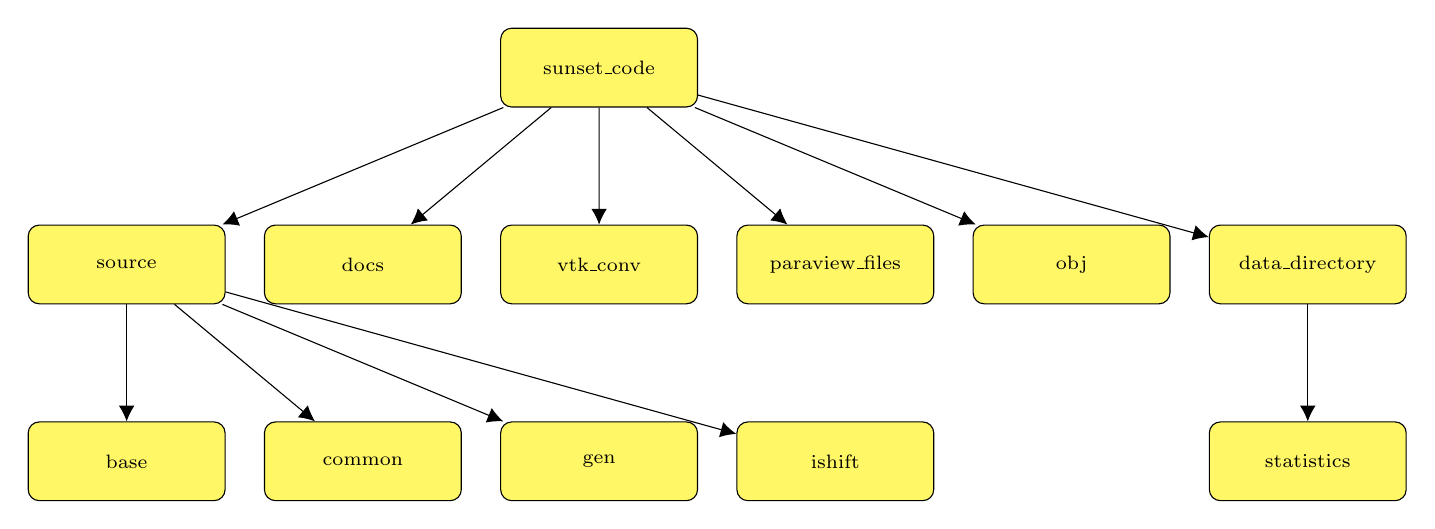
\begin{tikzpicture}[node distance=1.5cm,
    every node/.style={fill=white, font=\sffamily}, align=center]
  % Specification of nodes (position, etc.)
  \node (sph)       [box, xshift=6cm]                        {sunset\_code};
  \node (source)     [box, below of=sph, xshift=-6cm, yshift=-1cm]                  {source};
  \node (docs)    [box, right of=source, xshift=1.5cm]  {docs};
  \node (vtk)      [box, right of=docs, xshift=1.5cm]                {vtk\_conv};
  \node (parav)    [box, right of=vtk, xshift=1.5cm]     {paraview\_files};
  \node (obj)   [box, right of=parav, xshift=1.5cm]  {obj}; 
  \node (data)   [box, right of=obj, xshift=1.5cm]  {data\_directory};   
  
  \node (base)   [box, below of=source, yshift=-1cm]  {base};
  \node (common)   [box, right of=base, xshift=1.5cm]  {common};
  \node (gen)   [box, right of=common, xshift=1.5cm]  {gen};    
  \node (ishift) [box, right of=gen,xshift=1.5cm] {ishift};
  
  \node (stats)   [box, below of=data, yshift=-1cm]  {statistics};

  \draw[->] (sph) edge (source);
  \draw[->] (sph) edge (vtk);
  \draw[->] (sph) edge (parav);
  \draw[->] (sph) edge (data);
  \draw[->] (sph) edge (obj);        
  \draw[->] (sph) edge (docs);          

  \draw[->] (source) edge (base);
  \draw[->] (source) edge (common);
  \draw[->] (source) edge (gen);    
  \draw[->] (source) edge (ishift);   
    
  \draw[->] (data) edge (stats);        
  \end{tikzpicture}
  
\begin{itemize}
\item \verb|source| contains source files for the code:
\begin{itemize}
\item \verb|base| contains main modules for \verb|sunset_code|
\item \verb|para| contains parameters and common variables
\item \verb|gen| contains code to generate casefiles and initial conditions
\end{itemize}
\item \verb|vtk_conv| contains a program to convert output files into \verb|.vtu| files, which can be read by Paraview.
\item \verb|paraview_files| the program in \verb|vtk_conv| creates \verb|.vtu| files here.
\item \verb|obj| contains \verb|.o| and \verb|.mod| files created during compilation.
\item \verb|docs| contains this document and associated files.
\item \verb|data_directory| contains output files produced by the code. \verb|statistics| contains files describing global, time-varying measures (e.g. total K.E.).
\end{itemize}  

\bibliographystyle{elsarticle-num-names}
\bibliography{sunset_refs}

\end{document}


